\documentclass[aspectratio=169]{beamer}
\usepackage[english]{babel}
\usepackage{amsmath,amsfonts}
\usepackage{multicol}

\usepackage{IEEEtrantools}
\usepackage{multirow}
% beamer setup

%\usecolortheme{dove}

\setbeamertemplate{navigation symbols}{}
\setbeamertemplate{itemize items}[ball]

\usepackage{tikz}
\usetikzlibrary{shapes,arrows}
\usetikzlibrary{positioning}
\tikzstyle{block} = [rectangle, draw, rounded corners]
\tikzstyle{line} = [draw, -latex']

\DeclareMathOperator*{\argmin}{argmin}
\DeclareMathOperator*{\argmax}{argmax}
\DeclareMathOperator{\E}{\mathbb{E}}
\DeclareMathOperator{\I}{\mathbb{I}}

\AtBeginSection[]{
  \begin{frame}[plain]
  \addtocounter{framenumber}{-1}
  \vfill
  \centering
  %\begin{beamercolorbox}[sep=8pt,center,shadow=true,rounded=true]{title}
    %\usebeamerfont{title}
    \Huge{\insertsectionhead\par}%
  %\end{beamercolorbox}
  \vfill
  \end{frame}
}


\newcommand{\backupbegin}{
   \newcounter{framenumberappendix}
   \setcounter{framenumberappendix}{\value{framenumber}}
}
\newcommand{\backupend}{
   \addtocounter{framenumberappendix}{-\value{framenumber}}
   \addtocounter{framenumber}{\value{framenumberappendix}} 
}




\title{Bargaining with Taste Shocks}
\author{Egor Kozlov}

\institute{
  Department of Economics\\
  Northwestern University}
  
  
\setbeamertemplate{footline}[frame number]

  
%  \usepackage{pgf}
%\logo{\pgfputat{\pgfxy(0,0)}{\pgfbox[right,base]{\footnotesize{\insertframenumber\,/\,\inserttotalframenumber}}}}
%\newcommand{\nologo}{\setbeamertemplate{logo}{}}

\let\olditem\item
\renewcommand{\item}{%
\olditem\vspace{\fill}} 

\begin{document}



\begin{frame}[plain]
\addtocounter{framenumber}{-1}
\date{\scriptsize}
\titlepage
\end{frame}


\begin{frame}
\frametitle{Goal}
\begin{itemize}
\item This is a technical note
\item I try add taste shocks to the limited commitment model so the value functions are more smooth
\item Non-smoothness is large problem: more points are needed to achieve accuracy, policy functions (like savings) are discontinuous
\item Smoothing discrete choices is cool and modern (machine learning guys confirm)
\item DC-EGM (Iskhakov et al) approach is promising
\end{itemize}
\end{frame}


\begin{frame}
\frametitle{Existing Approach}
Standard renegotiation problem (discretized):
\begin{itemize}
\item \textit{Discrete} set $\Theta$ of possible bargaining powers, one-dimensional, $\Theta \subset [0,1]$
\item $\Theta = \{\theta_1,...\theta_n\}$
\item Couple starts with some $\theta_k$ and values of singleness $V^{fs}$, $V^{ms}$ and values values $\{V^f_1,...,V^f_n\}$, $\{V^m_1,...,V^m_n\}$ on $\Theta$. Here $V_i^{h} = V^h(\theta_i)$ for $h \in \{f,m\}$.
\item Then nested choice:
\begin{itemize}
\item Divorce if $\not\exists i \ : \ V^f_i - V^{fs}  \geq 0\ \& \ V^m_i - V^{ms} \geq 0$
\item Otherwise: 
\begin{itemize}
\item keep current $\theta_{sq}$ if $V^f_{sq} - V^{fs} \geq 0\ \& \ V^m_{sq} - V^{ms} \geq 0$
\item otherwise renegotiate to $\theta_{r^*}$: $\Theta_r = \{\theta_r \in \Theta: V^f_r - V^{fs} \geq 0\ \& \ V^m_r - V^{ms} \geq 0\}$, pick $\theta_{r^*}$ from $\Theta_r$ that is the closest to initial $\theta_{sq}$
\end{itemize}
%\item Equivalent metrics: $\Rightarrow \max\limits_{i} \left[ \min\{ V^f_i - V^{fs}, V^m_i - V^{ms} \} \right] < 0$.
\end{itemize}
\end{itemize}
\end{frame}

\begin{frame}
\frametitle{Reformulation}
Define the Rawlsian surplus $M_i = \min \{ V^f_i - V^{fs}, V^m_i - V^{ms} \}$

\textbf{Egalitarian bargaining solution (EBS)}: $\max\limits_i \min \{ V^f_i - V^{fs}, V^m_i - V^{ms} \} = M_{ebs}$

The choice problem then is:
\begin{itemize}
\item Divorce if $\not\exists i \ : \ V^f_i - V^{fs}  \geq 0\ \& \ V^m_i - V^{ms} \geq 0 \ \ \ \Leftrightarrow \ \ \ \boxed{ \max\limits_i M_i = M_{\text{EBS}} < 0 }$
\item Otherwise: 
\begin{itemize}
\item keep current $\theta_{sq}$ if $V^f_{sq} - V^{fs} \geq 0\ \& \ V^m_{sq} - V^{ms} \geq 0 \ \ \  \Leftrightarrow \ \ \ \boxed{ M_{sq} \geq 0 }$
\item otherwise renegotiate to $\theta_{r^*}$: $\Theta_R = \{\theta_r \in \Theta \ : \ V^f_r - V^{fs} \geq 0\ \& \ V^m_r - V^{ms} \geq 0\}$, pick $\theta_{r^*}$ from $\Theta_R$ that is the closest to initial $\theta_{sq}$. Equivalent representation: 
\[ \boxed{ \Theta_R = \{\theta_r \in \Theta \ : M_r \geq 0 \}. \ \ \theta_{r^*} \text{ is the closest value to $\theta_{sq}$ from $\Theta_R$ } }\]
\end{itemize}
\end{itemize}
\end{frame}

\begin{frame}
\frametitle{Single-Crossing Assumption in Renegotiation}
\begin{itemize}
\item \textbf{Assumption:} $V^f(\theta)$ and $V^m(\theta)$ are monotonic in $\theta$
\item \textbf{Then:} $M(\theta) = \min \{ V^f(\theta) - V^{fs}, V^m(\theta) - V^{ms} \}$ is single-crossing.
\item \textbf{Then:} If at $\theta_{sq}$ $M_{sq} < 0$ and $M_{ebs} > 0$, then $\theta_{sq} < \theta_{r^*}  < \theta_{ebs}$ (WLOG $\theta_{sq} < \theta_{\text{EBS}}$)
\item In real calculations, monotonicity can be violated (slightly). I hope that smoothing fixes this.
\item Two cases: $S^h = V^h(\theta) - V^{hs}$, $h \in \{f,m\}$
\end{itemize}

\begin{center}
\begin{tabular}{c c}
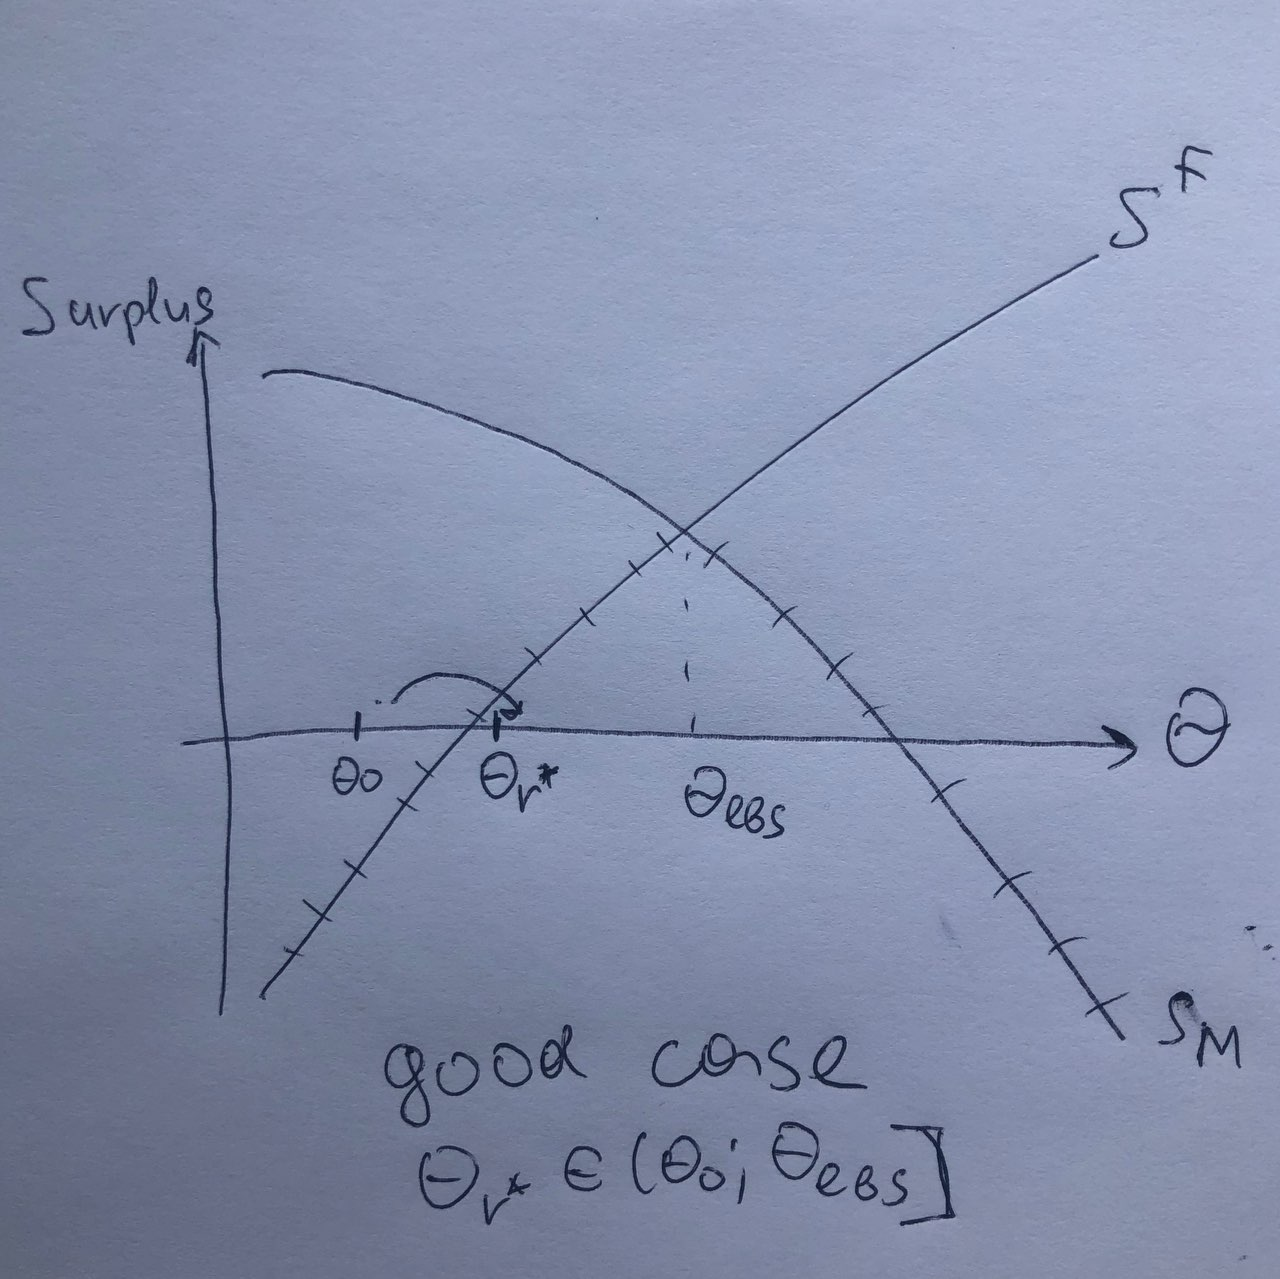
\includegraphics[scale=0.11]{m_good.jpg} & 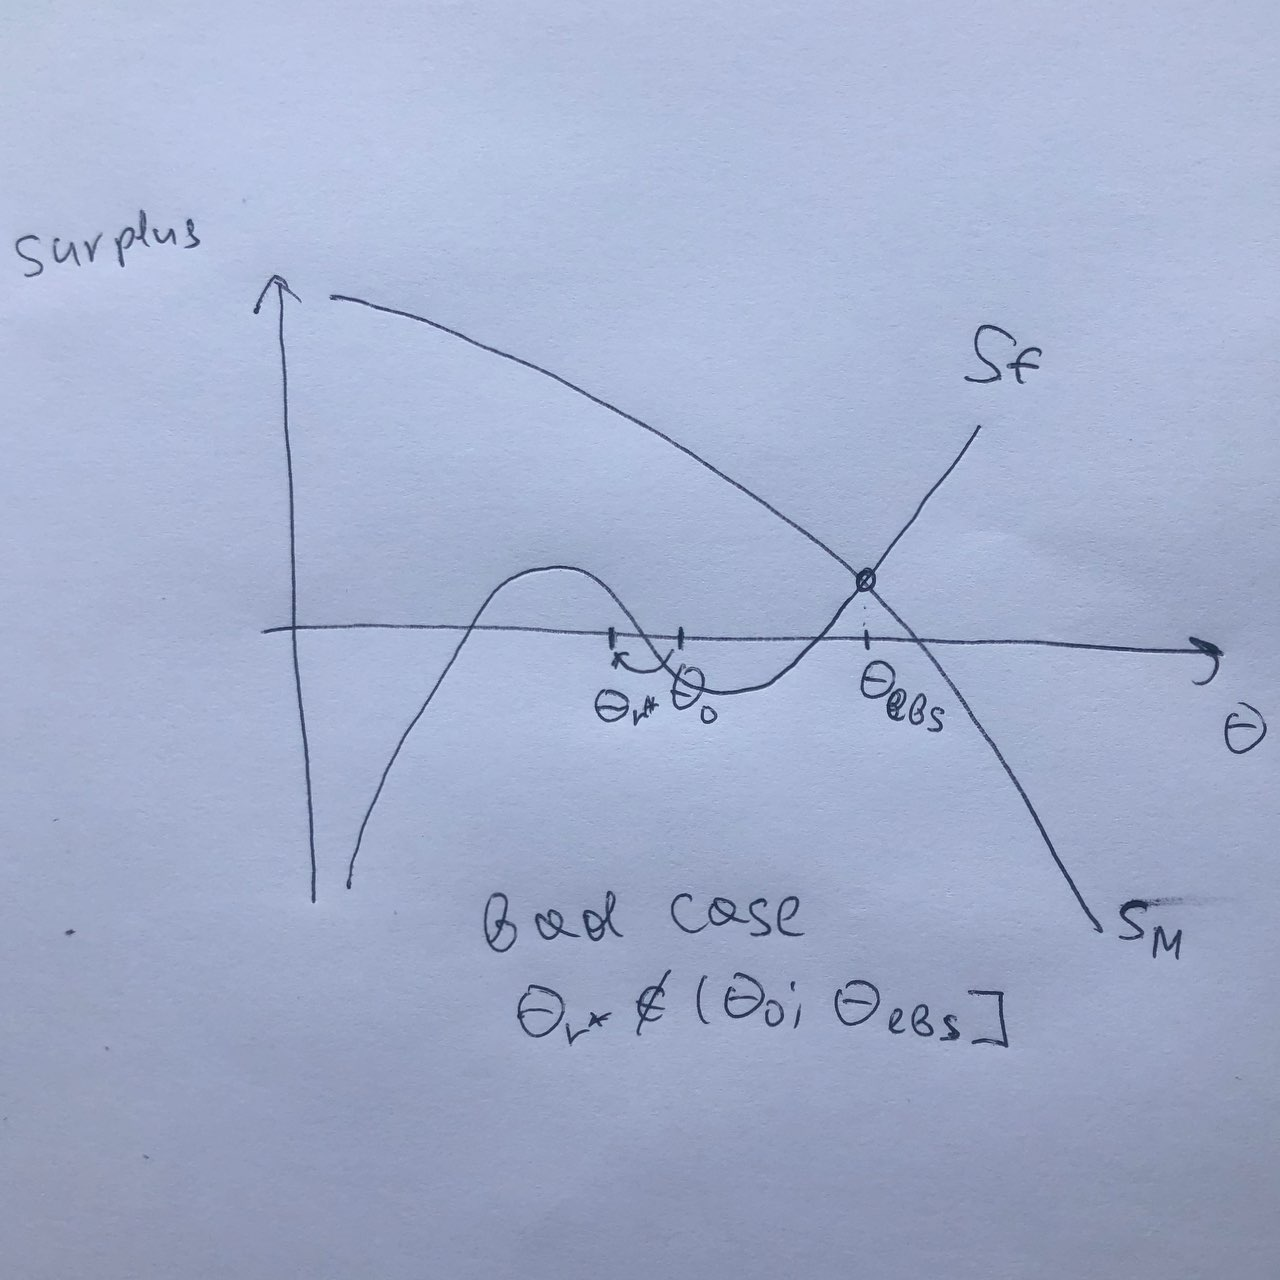
\includegraphics[scale=0.11]{m_bad.jpg} 
\end{tabular}
\end{center}
\end{frame}

\begin{frame}
\frametitle{Introducing Taste Shocks}
\begin{itemize}
\item Let $\xi$ is a shock to both partners' outside options. Participation constraints:
\[V^{f}(\theta) \geq V^{fs} + \xi, \ \ V^{m}(\theta) \geq V^{ms} + \xi.\]
\[S^f(\theta) = V^{f}(\theta) - V^{fs}, \ \ S^m = V^{m}(\theta) - V^{ms}, \ \ M(\theta) = \min\{S^f(\theta),S^m(\theta)\}.\]
Couple's decisions given $\xi$ are:
\begin{itemize}
\item Divorce if $\forall i \ \ M_i < \xi \ \ \Rightarrow \boxed{\xi > M_{ebs}}$
\item Stay together when having $\theta_k$ if $\boxed{\xi < M_k}$. Note that $M_k \leq M_{ebs}$.
\item Renegotiate current $\theta$ if $\xi \in (M_{sq}, M_{ebs})$. In this case, \textit{assuming single-crossing}, there exist two monotonic sequences from values of $\theta \in \Theta$:
\[ \theta_{sq} < \theta_{r_1} < ... < \theta_{r_h} < \theta_{ebs} \text{\ \ and \ \ } M_{sq} < M_{r_1} < ... < M_{r_h} < M_{ebs}.\]
$\theta_{r_k}$ is picked if $M_{r_{k-1}} < \xi < M_{r_k}$.
\end{itemize}
\end{itemize}
\end{frame}


\begin{frame}
\frametitle{Taste Shocks Create Distribution Over $\{\theta_{sq},\theta_1,\theta_2,\theta_3,\theta_{ebs},\text{divorce}\}$}
\begin{center}
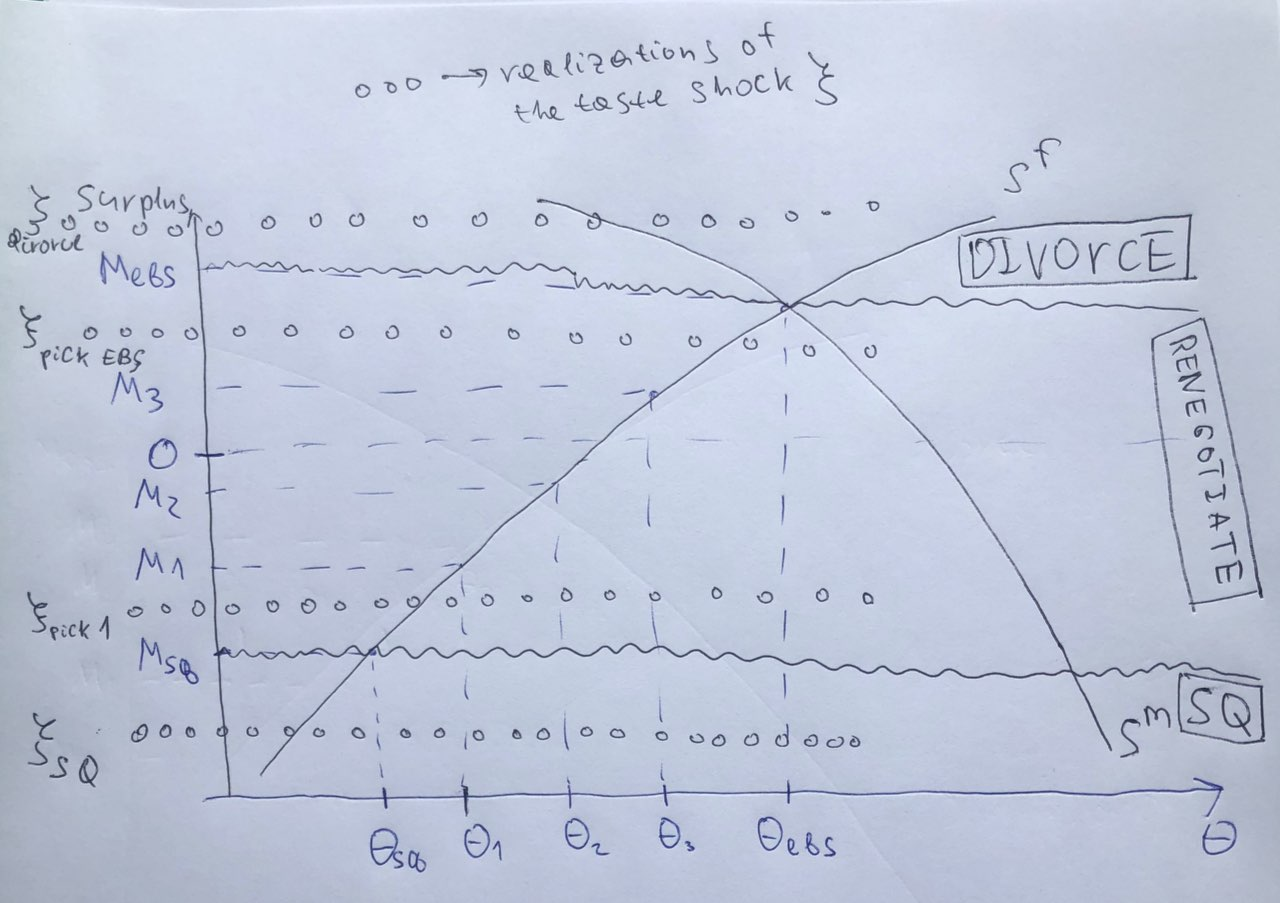
\includegraphics[scale=0.25]{taste_shocks.jpg}
\end{center}
\end{frame}

\begin{frame}
\frametitle{Renegotiation: Summary}
\begin{itemize}
\item With the taste shocks: 
\begin{itemize}
\item $P(\text{divorce}) = P(\xi > M_{ebs})$, $P(\text{keep sq: }\theta = \theta_{sq}) = P(\xi < M_{sq})$
\item $P(\text{renegotiate: }\theta = \theta_{r_j}) = P(M_{r_{j-1}} < \xi < M_{r_j})$, $P(\text{other $\theta$'s}) = 0$
\end{itemize}
\item When single crossing is violated, all prettiness goes away. Assume it is not...
\item Let $\theta_0 = \theta_{sq}$ and $\theta_{h+1} = \theta_{ebs}$, $M_{h+1} = M_{ebs}$ and $M_0 = M_{sq}$ 
\item Expected value function with this transition is:
\begin{align*}& \E_\xi \left[ \I(\xi < M_{sq}) V(\theta_{sq}) + \sum\limits_{j=1}^{h+1} \I(M_{j-1} < \xi < M_j) V(\theta_j) + \I(\xi>M_{ebs})(V^{\text{div}} + \xi) \right] = \\
& \ \ \Lambda_\xi (M_{sq}) V(\theta_{sq}) + (\Lambda_\xi(M_{j}) - \Lambda_{\xi}(M_{j-1})) V_{\theta_j} + (1-\Lambda(M_{ebs}))\cdot [V^{\text{div}} + \E(\xi|\xi>M_{ebs})].
 \end{align*}
Here $\Lambda_\xi(t) = \left[1 + \exp\left( t / \sigma_{\xi} \right)\right]^{-1}$. As $\sigma_\xi \to 0$ this convegres to $\I(t < 0)$.
\end{itemize}
\end{frame}


\begin{frame}
\frametitle{Adding Marriage is Simple}
\begin{itemize}
\item All the setup calls for egalitarian bargaining instead of Nash Bargaining Solution
\item Unlike $\theta_{nbs}$ that requires positive surplus, $\theta_{ebs}$ is always well-defined
\item When couple meet they pick $\theta = \theta_{ebs}$ and get common taste shock $-\zeta$
\item Agreement happens if $\min\{V^{f}_{ebs} - V^{fs} - \zeta, V^m_{ebs} - V^{ms} - \zeta \} > 0 \Leftrightarrow M_{ebs} > \zeta$
\item Expected value function (for the female) is then
\begin{align*}&\E_{\zeta} \left[ \I(\zeta < M_{ebs})(V^f - \zeta) + \I(\zeta > M_{ebs}) V^{fs} \right] = \\
& \ \ \Lambda_\zeta(M_{ebs}) \cdot \left[ V^f - \E(\zeta|\zeta<M_{ebs})\right] + \left[1-\Lambda_\zeta(M_{ebs})\right]\cdot V^{fs}
\end{align*}
\end{itemize}
\end{frame}


\begin{frame}
\frametitle{Conclusions}
\begin{itemize}
\item This smoothing can fix numeric problems and is relatively easy to implement.
\item Potentially it can allow to use Euler equation based methods (EGM) in the limited commitment models and save large chunk of time by avoiding expensive optimization. This requires thinking but is already doable.
\item Even without Euler equations it should make value function iteration more stable
\item I should be writing
\end{itemize}
\end{frame}



\end{document}


